\chapter{系统理论设计和仿真}

本章利用前文描述的基础知识,对基于压缩感知的太阳能组件缺陷检测系统进行理论
设计和数值仿真。首先设计压缩感知系统的核心——测量矩阵 $\Phi$ ,之后以小波域
的 $\ell_1$ 范数优化(Lasso 回归)和空间域的全变分优化方法为例进行数值仿真
实验,以验证采用压缩感知方法检测太阳能组件缺陷的可行性。

\section{感知系统理论设计}

目前的压缩感知理论框架要求线性测量,非线性的稀疏恢复理论尚未成型。根据式
\ref{eqn:LightCurrent} 知道,光电流与面积 $A$ ,以及光通量 $L$ 成正比。
这说明,我们可以采用不同强度的光照射太阳能电池板感光面的各个不同位置,
总的光电流就是各个位置产生的光电流之和:
\begin{equation}
I_L = \sum_i I_i = \sum_i (W_i K_i)  L_i(q_e \cdot \delta A)
\end{equation}
这里 $\delta A$ 是小面积元的大小,而 $(W_i K_i)$ 衡量了位置 $i$ 的光电
转化效率。这个式子就相当于光电转化效率和 $L_i$ 的内积。进行多次测量,每次
采用一组不同的 $L_i$ 。于是, $L_i$ 就相当于测量矩阵 $H$ 中的行,
$I_L$ 就是 $y$ 中的一个采样点。

为了获得光电流的大小,我们需要采用输入阻抗趋于 $0$ 的互阻型放大器 (I-V
变换器)对太阳能电池的输出电流进行放大。此时太阳能电池几乎短路,根据式
\ref{eqn:SCCurrent} 知道,输出电流的大小等于光电流。如果放大器前级的输出
阻抗不接近 $0$ ,根据式 \ref{eqn:Shockley} 和 \ref{eqn:TotalCurrent} 知道,
测得的总电流和光电流之间存在指数关系,导致测量结果严重非线性,就不能应用
压缩感知理论。

注意到矩阵中的每一行相当于一组光通量,为简单起见,采用 Bernoulli 矩阵作为
测量矩阵 $H$ 。由于 Bernoulli 矩阵中各个元素相互独立,服从两点($0-1$)
分布,即使光电流与光通量并不严格线性,也不会导致无法恢复。

我们试用两种恢复算法对 $x$ 进行恢复。第一种方法是直接采用全变分最小化方法
(求解问题 \ref{prob:TVopt})恢复 $x$:
\begin{equation}
\hat x = \mathop{\arg\min}_{x'} TV(x') \quad s.t. \quad
\|Hx' - y\|_2 \leq \epsilon
\end{equation}

另一方面,考虑到某些缺陷的边界并不是非常尖锐,采用全变分最小化可能效果
不佳,尝试使用小波基 $\Psi$ 展示 $x$ 的稀疏性:
\begin{equation}
y = Hx = H\Psi a
\end{equation}
定义 $\Phi = H\Psi$,通过 Lasso 回归(求解问题 \ref{prob:Lasso})恢复
稀疏表示 $a$,进而恢复 $x$:
\begin{equation}
\hat x = \Psi \hat a = \Psi \mathop{\arg\min}_{a'} \|a'\|_1 \quad s.t.
\quad \|\Phi a' - y\|_2 \leq \epsilon
\end{equation}
注意到根据定理 \ref{th:RandomRIP},当 $H$ 的行数 $M$ 足够大时,矩阵 $\Phi$
以约束等距常数 $\delta_{2K} < 1/3$ 满足 $2K$ 阶 RIP。又根据定理
\ref{th:l1recovery} ,Lasso 回归能够以有限误差重构稀疏表示 $a$。

测量系统的框图如图 \ref{fig:system} 所示。

\begin{figure}
\centering
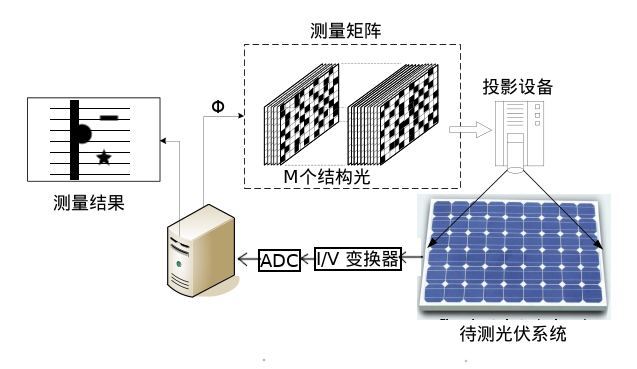
\includegraphics[width=.8\textwidth]{Figure/system.pdf}
\caption{测量系统框图}
\label{fig:system}
\end{figure}

下面我们将对这两种算法进行数值仿真,以比较它们的优劣。

\section{数值仿真}

\subsection{测试用例设计}

为了测试恢复算法的性能,需要设计一些具有代表性的测试用例。这里我们不深究
太阳能组件缺陷的产生原因,仅仅考虑缺陷的形态学特性。缺陷大致可以分为
坏点、裂纹和坏块,图 \ref{fig:testdata} 中的测试用例涵盖了这三种缺陷,
以及栅状电极的影响。

\begin{figure}
\centering
\begin{subfigure}[t]{1.1in}
	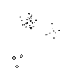
\includegraphics{Figure/testdata/0d.png}
	\caption{坏点}
	\label{fig:testdata:0d}
\end{subfigure}
\begin{subfigure}[t]{1.1in}
	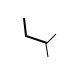
\includegraphics{Figure/testdata/1d.png}
	\caption{裂纹}
	\label{fig:testdata:1d}
\end{subfigure}
\begin{subfigure}[t]{1.1in}
	
\includegraphics{Figure/testdata/2dsharp.png}
	\caption{边缘清晰的坏块}
\end{subfigure}
\begin{subfigure}[t]{1.1in}
	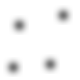
\includegraphics{Figure/testdata/2dsmooth.png}
	\caption{边缘模糊的坏块}
	\label{fig:testdata:2dsmooth}
\end{subfigure}
\begin{subfigure}[t]{1.1in}
	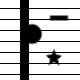
\includegraphics{Figure/testdata/2dsharp_finger.png}
	\caption{坏块与栅状电极}
\end{subfigure}
\caption{测试用例}
\label{fig:testdata}
\end{figure}

仿真中使用的随机矩阵 $H$ 为 Bernoulli 随机矩阵,其每一行均被标准化,使得
其 $\ell_2$ 范数为 $1$ ,均值为 $0$ 。这是多数压缩感知稀疏恢复算法对
测量矩阵的要求。 在实际测量中,我们不可能产生负的光通量,因此需要对采样数据
进行预处理,才能用恢复算法进行求解。

为了模拟实际测量时必然存在的噪声影响,我们为每组采样数据叠加 $10\%$ 的高斯
白噪声。由于 $H$ 的各行是归一化的,对采样数据增加噪声和对原始数据增加噪声
具有等价性。

$\ell1$ 最小化重建仿真中使用的小波基来自 \verb|ltfat| 软件包,其滤波器组为
$8$ 阶 Daubechies 滤波器,迭代次数为 $4$ 次\cite{ltfatnote015} 
\cite{ltfatnote030} 。

\subsection{全变分最小化重建的仿真结果}

全变分最小化重建均使用 Li 编写的 \verb|TVAL3| 软件包完成。该软件包
采用增广拉格朗日乘子法和交替方向算法求解全变分最小化重建问题,是一款非常
优秀的全变分最小化求解器。关于该软件包的设计思路和实现细节,参见文献
\cite{TVAL3CBLMaster} \cite{TVAL3CBLPhD}。

对坏点(图 \ref{fig:testdata:0d} )的重建结果如图 \ref{fig:TV0d} 所示。

\begin{figure}
\centering
\begin{subfigure}[t]{1.1in}
	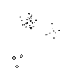
\includegraphics{Figure/testdata/0d.png}
	\caption{原始数据}
\end{subfigure}
\begin{subfigure}[t]{1.1in}
	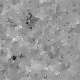
\includegraphics{Figure/TV/0d10.png}
	\caption{$M = 0.1 N$}
\end{subfigure}
\begin{subfigure}[t]{1.1in}
	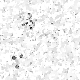
\includegraphics{Figure/TV/0d30.png}
	\caption{$M = 0.3 N$}
\end{subfigure}
\begin{subfigure}[t]{1.1in}
	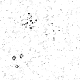
\includegraphics{Figure/TV/0d50.png}
	\caption{$M = 0.5 N$}
\end{subfigure}
\begin{subfigure}[t]{1.1in}
	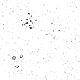
\includegraphics{Figure/TV/0d70.png}
	\caption{$M = 0.7 N$}
\end{subfigure}
\caption{坏点的全变分最小化重建结果}
\label{fig:TV0d}
\end{figure}

可见, $M = 0.1 N$ 时重建完全失败,这是由于 $M$ 太小,不满足定理
\ref{th:RandomRIP} 的要求,导致矩阵 $H$ 丧失 RIP 性质。

对裂纹(图 \ref{fig:testdata:1d} )的重建结果如图 \ref{fig:TV1d} 所示。

\begin{figure}
\centering
\begin{subfigure}[t]{1.1in}
	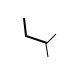
\includegraphics{Figure/testdata/1d.png}
	\caption{原始数据}
\end{subfigure}
\begin{subfigure}[t]{1.1in}
	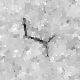
\includegraphics{Figure/TV/1d10.png}
	\caption{$M = 0.1 N$}
\end{subfigure}
\begin{subfigure}[t]{1.1in}
	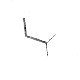
\includegraphics{Figure/TV/1d30.png}
	\caption{$M = 0.3 N$}
\end{subfigure}
\begin{subfigure}[t]{1.1in}
	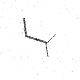
\includegraphics{Figure/TV/1d50.png}
	\caption{$M = 0.5 N$}
\end{subfigure}
\begin{subfigure}[t]{1.1in}
	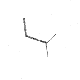
\includegraphics{Figure/TV/1d70.png}
	\caption{$M = 0.7 N$}
\end{subfigure}
\caption{裂纹的全变分最小化重建结果}
\label{fig:TV1d}
\end{figure}

除了 $M = 0.1N$ 时重建结果很差外,其他三次重建都较好地恢复了
图像中的裂纹。然而,可以注意到裂纹出现较为明显的锯齿,这是由于
全变分最小化会促进图像梯度的稀疏性,导致图像出现类似阶梯函数的
特性。

对边界清晰的坏块重建结果见图 \ref{fig:TV2dsharp}。
可以看出,全变分最小化对边界稀疏的图像重建效果很好,甚至只要
$10\%$ 的采样即可几乎完美地恢复出图像中的三个坏块。

\begin{figure}
\centering
\begin{subfigure}[t]{1.1in}
	
\includegraphics{Figure/testdata/2dsharp.png}
	\caption{原始数据}
\end{subfigure}
\begin{subfigure}[t]{1.1in}
	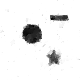
\includegraphics{Figure/TV/2dsharp10.png}
	\caption{$M = 0.1 N$}
\end{subfigure}
\begin{subfigure}[t]{1.1in}
	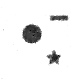
\includegraphics{Figure/TV/2dsharp30.png}
	\caption{$M = 0.3 N$}
\end{subfigure}
\begin{subfigure}[t]{1.1in}
	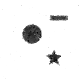
\includegraphics{Figure/TV/2dsharp50.png}
	\caption{$M = 0.5 N$}
\end{subfigure}
\begin{subfigure}[t]{1.1in}
	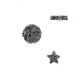
\includegraphics{Figure/TV/2dsharp70.png}
	\caption{$M = 0.7 N$}
\end{subfigure}
\caption{边界清晰坏块的全变分最小化重建结果}
\label{fig:TV2dsharp}
\end{figure}

对边界模糊的坏块重建结果如图 \ref{fig:TV2dsmooth}
所示。重建结果很差,这是由于图像
\ref{fig:testdata:2dsmooth} 的梯度并不十分稀疏,导致定理
\ref{th:RandomRIP} 的条件难以满足。可见,全变分最小化方法不适合
恢复颜色变化较为平滑的图像。

\begin{figure}
\centering
\begin{subfigure}[t]{1.1in}
	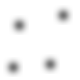
\includegraphics{Figure/testdata/2dsmooth.png}
	\caption{原始数据}
\end{subfigure}
\begin{subfigure}[t]{1.1in}
	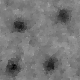
\includegraphics{Figure/TV/2dsmooth10.png}
	\caption{$M = 0.1 N$}
\end{subfigure}
\begin{subfigure}[t]{1.1in}
	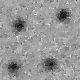
\includegraphics{Figure/TV/2dsmooth30.png}
	\caption{$M = 0.3 N$}
\end{subfigure}
\begin{subfigure}[t]{1.1in}
	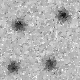
\includegraphics{Figure/TV/2dsmooth50.png}
	\caption{$M = 0.5 N$}
\end{subfigure}
\begin{subfigure}[t]{1.1in}
	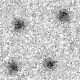
\includegraphics{Figure/TV/2dsmooth70.png}
	\caption{$M = 0.7 N$}
\end{subfigure}
\caption{边界模糊坏块的全变分最小化重建结果}
\label{fig:TV2dsmooth}
\end{figure}

对栅状电极的重建结果如图 \ref{fig:TVfinger}
所示。可以看出,栅状电极的存在严重破坏了梯度的稀疏性,导致
全变分最小化恢复过程需要更多的采样数据。

\begin{figure}
\centering
\begin{subfigure}[t]{1.1in}
	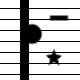
\includegraphics{Figure/testdata/2dsharp_finger.png}
	\caption{原始数据}
\end{subfigure}
\begin{subfigure}[t]{1.1in}
	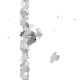
\includegraphics{Figure/TV/finger10.png}
	\caption{$M = 0.1 N$}
\end{subfigure}
\begin{subfigure}[t]{1.1in}
	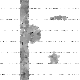
\includegraphics{Figure/TV/finger30.png}
	\caption{$M = 0.3 N$}
\end{subfigure}
\begin{subfigure}[t]{1.1in}
	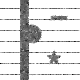
\includegraphics{Figure/TV/finger50.png}
	\caption{$M = 0.5 N$}
\end{subfigure}
\begin{subfigure}[t]{1.1in}
	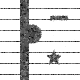
\includegraphics{Figure/TV/finger70.png}
	\caption{$M = 0.7 N$}
\end{subfigure}
\caption{坏块与栅状电极的全变分最小化重建结果}
\label{fig:TVfinger}
\end{figure}

\subsection{$\ell_1$ 范数最小化重建的仿真结果}

$\ell_1$ 范数最小化重建采用 Zhang 等编写的 \verb|YALL1| 软件包完成。该
软件包功能强大,可求解多种形式的 $\ell_1$ 优化问题。和 \verb|TVAL3| 一样,
该软件包也采用交替方向算法进行最优化求解,运行效率较高,能够高效地完成
数值仿真。

图 \ref{fig:l10d} 给出了坏点仿真数据(图 
\ref{fig:testdata:0d} )的 $\ell_1$ 最小化恢复结果。

\begin{figure}
\centering
\begin{subfigure}[t]{1.1in}
	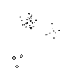
\includegraphics{Figure/testdata/0d.png}
	\caption{原始数据}
\end{subfigure}
\begin{subfigure}[t]{1.1in}
	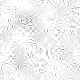
\includegraphics{Figure/L1/0d10.png}
	\caption{$M = 0.1 N$}
\end{subfigure}
\begin{subfigure}[t]{1.1in}
	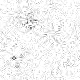
\includegraphics{Figure/L1/0d30.png}
	\caption{$M = 0.3 N$}
\end{subfigure}
\begin{subfigure}[t]{1.1in}
	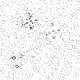
\includegraphics{Figure/L1/0d50.png}
	\caption{$M = 0.5 N$}
\end{subfigure}
\begin{subfigure}[t]{1.1in}
	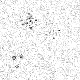
\includegraphics{Figure/L1/0d70.png}
	\caption{$M = 0.7 N$}
\end{subfigure}
\caption{坏点的 $\ell_1$ 最小化重建结果}
\label{fig:l10d}
\end{figure}

可见, $M = 0.1 N$ 时重建仍然完全失败。由于小波变换并不能增加坏点图像的
稀疏性,此时测量矩阵 $\Phi = H \Psi$ 同全变分最小化求解时使用的矩阵 $H$
一样,不满足 RIP 条件。因此,$M = 0.1N$ 时,无论采用何种算法,只要无法
在某个字典下稀疏表示坏点,都几乎不可能成功重建图像。

$M$ 较大时则可以成功重建图像,但是注意到 $M=0.7$ 时的重建结果中,噪点比
$M=0.5$ 时更多,直观上图像质量发生了退化。这是由于 $\Phi$ 规模的增加
加强了 Lasso 回归的约束条件:
\begin{equation}
\|\Phi a' - y\|_2 \leq \epsilon
\end{equation}
从而降低了 $\ell_1$ 优化的自由度,导致 $\ell_1$ 最小化本身具有的降噪功能
难以充分发挥。

图 \ref{fig:L11d} 给出针对裂纹的测试数据(图 \ref{fig:testdata:1d} )
的重建结果。

\begin{figure}
\centering
\begin{subfigure}[t]{1.1in}
	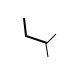
\includegraphics{Figure/testdata/1d.png}
	\caption{原始数据}
\end{subfigure}
\begin{subfigure}[t]{1.1in}
	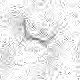
\includegraphics{Figure/L1/1d10.png}
	\caption{$M = 0.1 N$}
\end{subfigure}
\begin{subfigure}[t]{1.1in}
	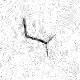
\includegraphics{Figure/L1/1d30.png}
	\caption{$M = 0.3 N$}
\end{subfigure}
\begin{subfigure}[t]{1.1in}
	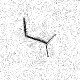
\includegraphics{Figure/L1/1d50.png}
	\caption{$M = 0.5 N$}
\end{subfigure}
\begin{subfigure}[t]{1.1in}
	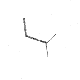
\includegraphics{Figure/TV/1d70.png}
	\caption{$M = 0.7 N$}
\end{subfigure}
\caption{裂纹的 $\ell_1$ 最小化重建结果}
\label{fig:L11d}
\end{figure}

除了 $M = 0.1N$ 时重建结果很差外,其他三次重建都较好地恢复了
图像中的裂纹。

对边界清晰的坏块重建结果见图 \ref{fig:L12dsharp}。
可以看出,边界稀疏图像更适合采用全变分最小化恢复, $\ell_1$ 恢复
求解的结果在 $M$ 较小时较全变分方法更差。

\begin{figure}
\centering
\begin{subfigure}[t]{1.1in}
	
\includegraphics{Figure/testdata/2dsharp.png}
	\caption{原始数据}
\end{subfigure}
\begin{subfigure}[t]{1.1in}
	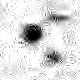
\includegraphics{Figure/L1/2dsharp10.png}
	\caption{$M = 0.1 N$}
\end{subfigure}
\begin{subfigure}[t]{1.1in}
	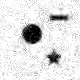
\includegraphics{Figure/L1/2dsharp30.png}
	\caption{$M = 0.3 N$}
\end{subfigure}
\begin{subfigure}[t]{1.1in}
	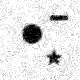
\includegraphics{Figure/L1/2dsharp50.png}
	\caption{$M = 0.5 N$}
\end{subfigure}
\begin{subfigure}[t]{1.1in}
	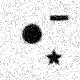
\includegraphics{Figure/L1/2dsharp70.png}
	\caption{$M = 0.7 N$}
\end{subfigure}
\caption{边界清晰坏块的 $\ell_1$ 最小化重建结果}
\label{fig:L12dsharp}
\end{figure}

对边界模糊的坏块重建结果如图 \ref{fig:L12dsmooth}
所示。重建结果与全变分最小化的结果相比较好,因为小波变换相比于求梯度能更好
地增加该图像的稀疏性。然而,横向比较表明,重建结果仍然不如其他测试数据,说
明仍需进行进一步研究,寻找能够稀疏表示边界模糊坏块的字典。

\begin{figure}
\centering
\begin{subfigure}[t]{1.1in}
	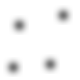
\includegraphics{Figure/testdata/2dsmooth.png}
	\caption{原始数据}
\end{subfigure}
\begin{subfigure}[t]{1.1in}
	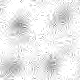
\includegraphics{Figure/L1/2dsmooth10.png}
	\caption{$M = 0.1 N$}
\end{subfigure}
\begin{subfigure}[t]{1.1in}
	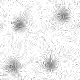
\includegraphics{Figure/L1/2dsmooth30.png}
	\caption{$M = 0.3 N$}
\end{subfigure}
\begin{subfigure}[t]{1.1in}
	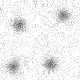
\includegraphics{Figure/L1/2dsmooth50.png}
	\caption{$M = 0.5 N$}
\end{subfigure}
\begin{subfigure}[t]{1.1in}
	\includegraphics{Figure/L1/2dsmooth70.png}
	\caption{$M = 0.7 N$}
\end{subfigure}
\caption{边界模糊坏块的 $\ell_1$ 最小化重建结果}
\label{fig:L12dsmooth}
\end{figure}

对栅状电极的重建结果如图 \ref{fig:L1finger}
所示。 栅状电极的存在也严重破坏了图像在小波字典下的稀疏性,直到 $M = 0.5N$
时才能够较好地恢复图像。

\begin{figure}
\centering
\begin{subfigure}[t]{1.1in}
	\includegraphics{Figure/testdata/2dsharp_finger.png}
	\caption{原始数据}
\end{subfigure}
\begin{subfigure}[t]{1.1in}
	\includegraphics{Figure/L1/finger10.png}
	\caption{$M = 0.1 N$}
\end{subfigure}
\begin{subfigure}[t]{1.1in}
	\includegraphics{Figure/L1/finger30.png}
	\caption{$M = 0.3 N$}
\end{subfigure}
\begin{subfigure}[t]{1.1in}
	\includegraphics{Figure/L1/finger50.png}
	\caption{$M = 0.5 N$}
\end{subfigure}
\begin{subfigure}[t]{1.1in}
	\includegraphics{Figure/L1/finger70.png}
	\caption{$M = 0.7 N$}
\end{subfigure}
\caption{坏块与栅状电极的 $\ell_1$ 最小化重建结果}
\label{fig:L1finger}
\end{figure}

以上仿真结果表明,压缩感知方法确实可以检测太阳能电池中的缺陷,且采样次数
为对整个光学面采样的 $10\%$ 至 $50\%$ 。仿真结果是在较为理想的情况下得出的,
在实际工作中,文献 \cite{XDUCLBIC} 建议使用 $40\%$ 至 $60\%$ 的采样次数,
而文献 \cite{CLBIC17} 建议使用 $40\%$ 至 $80\%$。
